\documentclass{beamer}
\usepackage[utf8]{inputenc}
\usepackage[english]{babel}
\usepackage[T1]{fontenc}
\usepackage{slide_helper}
\usepackage[inline]{asymptote}
\usepackage{asy_helper}
\usepackage[super]{nth}
\usepackage{array}
\usepackage{wasysym}
\usepackage{pgfplots}
\pgfplotsset{compat=1.5} 
\usepgfplotslibrary{statistics}

\DeclareSymbolFont{extraup}{U}{zavm}{m}{n}
\DeclareMathSymbol{\varheart}{\mathalpha}{extraup}{86}
\DeclareMathSymbol{\vardiamond}{\mathalpha}{extraup}{87}
\DeclareMathSymbol{\varclub}{\mathalpha}{extraup}{84} 
\DeclareMathSymbol{\varspade}{\mathalpha}{extraup}{85}

\newcommand{\suitheart}[1][]{{\color{red}\text{#1}\varheart}}
\newcommand{\suitspade}[1][]{{\color{black}\text{#1}\spadesuit}}
\newcommand{\suitdiamond}[1][]{{\color{red}\text{#1}\vardiamond}}
\newcommand{\suitclub}[1][]{{\color{black}\text{#1}\varclub}}

\newcommand{\prob}[1]{P\left(#1\right)}
\newcommand{\condprob}[2]{\prob{#1~\middle|~#2}}
\newcommand{\comb}[2]{{_{#1}C_{#2}}}
\newcommand{\perm}[2]{_{#1}P_{#2}}

\newcommand{\nullhypothesis}[1]{H_0:~{#1}}
\newcommand{\althypothesis}[1]{H_A:~{#1}}

\begin{asydef}
real nd_func(real mu, real sigma, real x) { return 1/sqrt(2*pi*sigma*sigma)*exp((-1*(x-mu)*(x-mu))/(2*sigma*sigma)); }

guide normal_dist(real mu, real sigma, real xmin, real xmax)
{
	real f(real x) { return nd_func(mu, sigma, x); }
	return graph(f, xmin, xmax);
}

void shade_between(real mu, real sigma, real a, real b, pen p=orange)
{
	real f(real x) { return nd_func(mu, sigma, x); }
	guide g = graph(f, a, b);
	
	filldraw((a,0) -- g -- (b,0) -- cycle, p, black);
}

void multiple_nd_curves_example(real std_dev)
{
	size(300, 190, IgnoreAspect);
    
    draw(normal_dist(0, std_dev, -6,6));
    shade_between(0,std_dev,-std_dev,std_dev);
    draw((0,0)--(0,0.45));
    
    label("$\sigma="+format("%#.2f", std_dev)+"$", (-4.2,0.45), Fill(paleyellow));
    
    xaxis(Bottom(), RightTicks(new real[] {-6,-4,-2,0,2,4,6}));
    yaxis(Left(), LeftTicks(size=nan),ymin = 0, ymax = 0.5);
}
\end{asydef}

\begin{asydef}
pair crit = (150, 33);
real a=-1.25;
real b=1.25;
\end{asydef}

\title[MA205 - Section 10.1]{Correlation}

\begin{document}
\begin{frame}
\titlepage
\end{frame}

\begin{frame}\small
\begin{definition}
A \textbf{correlation} exists between two variables when the values of one variable are somehow associated with the values of the other variables.
\end{definition}\pause

\begin{definition}
A \textbf{linear correlation} exists between two variables when there is a correlation and the plotted points of paired data result in a pattern that can be approximated by a straight line.
\end{definition}\pause

\begin{definition}
A \textbf{scatterplot} is a plot of paired $(x,y)$ quantitative data with a horizontal x-axis and a vertical y-axis. The horizontal axis is used for the first variable ($x$), and the vertical axis for the second variable ($y$).
\end{definition}\pause

\begin{note}
Because conclusions based on visual examinations of scatterplots are largely subjective, we need more objective measures. We use the linear correlation coefficient $r$, which is a number that measures the strength of the linear association between the two variables.
\end{note}
\end{frame}

\begin{frame}
\begin{example}
\begin{center}
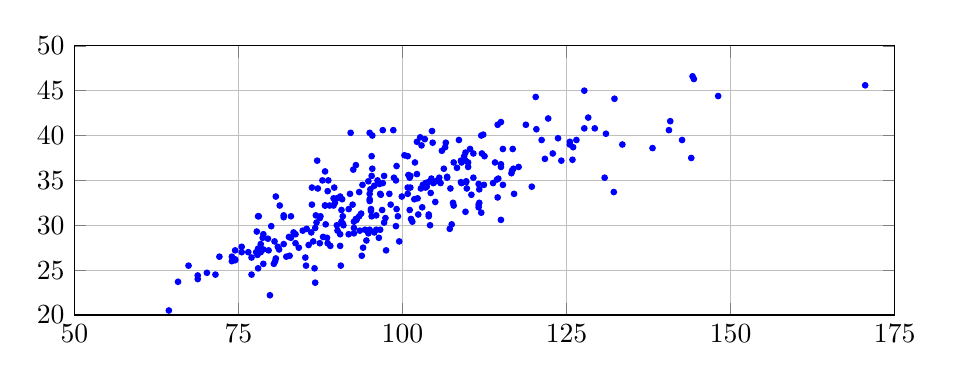
\begin{tikzpicture}
\pgfkeys{/pgf/number format/.cd,
fixed,
precision=999,
set thousands separator={},
1000 sep in fractionals=false,
}
\begin{axis}[
width=12cm,
height=5.0cm,
%xlabel={Waist Circumference (cm)},
%ylabel={Arm Circumference (cm)},
ymajorgrids=true,
xmajorgrids=true,
%enlarge x limits=false,
%enlarge y limits=false,
xticklabel style={/pgf/number format/.cd,fixed,precision=0},
xticklabel=\pgfmathprintnumber{\tick},
xtick={50,75,...,175},
ytick={20,25,...,50},
ymin=20,
ymax=50,
xmin=50,
xmax=175,
scatter/use mapped color={
 %draw=mapped color,
 fill=blue,
},
]
\addplot[scatter, only marks, blue, scatter src=y, mark size=1pt]
coordinates
{
(	120.4	,	40.7	)
(	107.8	,	37	)
(	120.3	,	44.3	)
(	97.2	,	30.3	)
(	95.1	,	34	)
(	112	,	31.4	)
(	78	,	27.4	)
(	103.5	,	34.2	)
(	89.7	,	32.5	)
(	112	,	40	)
(	95	,	32.7	)
(	115.3	,	38.5	)
(	118.8	,	41.2	)
(	92.6	,	30.4	)
(	75.5	,	27	)
(	101.8	,	32.9	)
(	92.5	,	36.2	)
(	100.8	,	33.5	)
(	82.8	,	26.6	)
(	92.9	,	36.7	)
(	109	,	34.7	)
(	101.9	,	37	)
(	110	,	36.5	)
(	102.3	,	33	)
(	80	,	29.9	)
(	94.3	,	29.5	)
(	103.1	,	34.5	)
(	103	,	32	)
(	90.5	,	29	)
(	88.2	,	36	)
(	78.8	,	29	)
(	65.8	,	23.7	)
(	114.4	,	35.1	)
(	78	,	25.2	)
(	106.8	,	35.4	)
(	112.4	,	34.5	)
(	94.8	,	34.9	)
(	90.6	,	25.5	)
(	95.2	,	31.8	)
(	71.5	,	24.5	)
(	94.5	,	28.3	)
(	95.3	,	31	)
(	103.5	,	34.7	)
(	104.2	,	30	)
(	88.7	,	35	)
(	109.7	,	34.9	)
(	115	,	36.8	)
(	64.4	,	20.5	)
(	133.5	,	39	)
(	102.2	,	39.3	)
(	138.1	,	38.6	)
(	112.1	,	38	)
(	70.2	,	24.7	)
(	144.4	,	46.3	)
(	95.7	,	29.2	)
(	98.7	,	35.3	)
(	121.7	,	37.4	)
(	87.4	,	28	)
(	77.7	,	27	)
(	100.9	,	35.6	)
(	93.4	,	33.7	)
(	125.9	,	37.3	)
(	121.2	,	39.5	)
(	90.5	,	27.7	)
(	86.7	,	23.6	)
(	82.3	,	26.5	)
(	107.3	,	34.1	)
(	88.2	,	32.2	)
(	129.3	,	40.8	)
(	78.8	,	25.7	)
(	95	,	29.5	)
(	102.8	,	34.1	)
(	85.3	,	25.5	)
(	79.6	,	27.2	)
(	101.2	,	34.2	)
(	111.6	,	32	)
(	90.8	,	32.9	)
(	108.6	,	39.5	)
(	81.9	,	30.9	)
(	132.2	,	33.7	)
(	87	,	37.2	)
(	108.9	,	37.2	)
(	74.5	,	27.2	)
(	107.7	,	32.5	)
(	96	,	29.5	)
(	79.5	,	28.5	)
(	111.7	,	34	)
(	83	,	28.6	)
(	80.6	,	26	)
(	102.4	,	31.2	)
(	96.7	,	33.4	)
(	93	,	30.6	)
(	88.6	,	28	)
(	97	,	40.6	)
(	95.4	,	36.3	)
(	104.5	,	40.5	)
(	106.3	,	36.3	)
(	97.2	,	35.5	)
(	140.8	,	41.6	)
(	90.5	,	33.2	)
(	98.6	,	40.6	)
(	115	,	41.5	)
(	98.2	,	32.3	)
(	114.5	,	33.1	)
(	108.9	,	34.8	)
(	80.7	,	26.3	)
(	96.9	,	31.7	)
(	95.4	,	40	)
(	100.8	,	37.7	)
(	99.1	,	36.6	)
(	88.6	,	33.8	)
(	87.8	,	35	)
(	105.6	,	35.3	)
(	103.4	,	39.6	)
(	116.6	,	35.8	)
(	85.7	,	27.8	)
(	90.9	,	30.2	)
(	89.5	,	33	)
(	89	,	27.7	)
(	77.8	,	29.3	)
(	77.9	,	26.7	)
(	104	,	31.2	)
(	105.1	,	34.9	)
(	84.8	,	29.4	)
(	127.7	,	40.8	)
(	81.9	,	31.1	)
(	126.5	,	39.5	)
(	83	,	31	)
(	96.4	,	28.6	)
(	106	,	38.3	)
(	83.7	,	29	)
(	101.2	,	35.5	)
(	96.2	,	35	)
(	104.6	,	39.2	)
(	77	,	24.5	)
(	115	,	30.6	)
(	86.1	,	29.2	)
(	102.2	,	35.7	)
(	93.9	,	34.5	)
(	92.4	,	32.3	)
(	110.3	,	38.5	)
(	127.7	,	45	)
(	99.1	,	31.8	)
(	109.8	,	34.1	)
(	95.2	,	31.6	)
(	99	,	29.9	)
(	87.9	,	28.7	)
(	123.7	,	39.7	)
(	107.2	,	29.6	)
(	86.4	,	28.2	)
(	90.7	,	30.4	)
(	68.8	,	24.4	)
(	68.8	,	24	)
(	99.3	,	31	)
(	140.6	,	40.6	)
(	119.7	,	34.3	)
(	83.7	,	28	)
(	96.6	,	33.5	)
(	99	,	35	)
(	88.2	,	32.2	)
(	87.5	,	31	)
(	81.9	,	27.9	)
(	97.5	,	27.2	)
(	106.6	,	39.2	)
(	91	,	30	)
(	80.4	,	25.7	)
(	107.8	,	32.2	)
(	76.5	,	27	)
(	115.3	,	34.5	)
(	95.3	,	35.5	)
(	109.6	,	38.1	)
(	110.8	,	38	)
(	92.9	,	30.7	)
(	114.5	,	41.2	)
(	109.6	,	37.2	)
(	122.9	,	38	)
(	78.8	,	27.3	)
(	92	,	33.5	)
(	99.5	,	28.2	)
(	114.6	,	35.2	)
(	90	,	30	)
(	87.1	,	34.1	)
(	93.5	,	29.4	)
(	170.5	,	45.6	)
(	105.8	,	34.7	)
(	100.3	,	37.8	)
(	92.6	,	29.7	)
(	88.3	,	30.1	)
(	110.5	,	33.4	)
(	102.7	,	39.8	)
(	112.5	,	37.7	)
(	105.4	,	35	)
(	132.3	,	44.1	)
(	104.3	,	33.6	)
(	94.8	,	29.1	)
(	85.4	,	29.6	)
(	96.5	,	34.6	)
(	109.6	,	31.5	)
(	106.5	,	38.7	)
(	79.8	,	22.2	)
(	84.2	,	27.5	)
(	89.5	,	32.2	)
(	90.1	,	29.4	)
(	116.8	,	38.5	)
(	148.1	,	44.4	)
(	93.4	,	31	)
(	77	,	26.4	)
(	116.7	,	36.1	)
(	101.5	,	30.4	)
(	112.3	,	40.1	)
(	96.6	,	29.5	)
(	83.4	,	29.2	)
(	81.3	,	32.2	)
(	144.2	,	46.6	)
(	103.7	,	34.3	)
(	95.7	,	34.4	)
(	81	,	27.6	)
(	126	,	38.7	)
(	89.6	,	34.2	)
(	98	,	33.5	)
(	110.8	,	35.3	)
(	104	,	31	)
(	99.9	,	33.2	)
(	95.3	,	37.7	)
(	105	,	32.6	)
(	131	,	40.2	)
(	125.5	,	39.3	)
(	80.7	,	33.2	)
(	110	,	37	)
(	130.8	,	35.3	)
(	78.7	,	28.6	)
(	97	,	34.7	)
(	88.9	,	32.2	)
(	90.7	,	31.7	)
(	86.9	,	30.3	)
(	95	,	32.9	)
(	80.5	,	28.2	)
(	104.4	,	35.2	)
(	74	,	26	)
(	104.7	,	34.7	)
(	101.3	,	30.7	)
(	82.7	,	28.7	)
(	115	,	36.5	)
(	72.1	,	26.5	)
(	95	,	40.3	)
(	96	,	31.1	)
(	87.4	,	30.8	)
(	111.7	,	32.5	)
(	111.6	,	32.3	)
(	74.5	,	26.2	)
(	128.3	,	42	)
(	102.9	,	38.9	)
(	108.3	,	36.4	)
(	94	,	27.5	)
(	81.2	,	27.3	)
(	122.2	,	41.9	)
(	75.5	,	27.6	)
(	109.4	,	37.7	)
(	91.8	,	29	)
(	114.1	,	37	)
(	124.2	,	37.2	)
(	111.6	,	34.6	)
(	116.9	,	36.3	)
(	86.8	,	31.1	)
(	86.6	,	25.2	)
(	86.2	,	32.3	)
(	92.6	,	29.1	)
(	109.7	,	34.8	)
(	106.8	,	35.3	)
(	93.8	,	26.6	)
(	100.8	,	34.2	)
(	117	,	33.5	)
(	78.4	,	27	)
(	86.7	,	29.7	)
(	91.8	,	31.8	)
(	85.2	,	26.4	)
(	93.7	,	31.3	)
(	144	,	37.5	)
(	113.8	,	34.7	)
(	103.9	,	34.8	)
(	95	,	33.5	)
(	78	,	31	)
(	101.1	,	35.3	)
(	107.5	,	30.1	)
(	97.4	,	30.8	)
(	90.9	,	31	)
(	88.5	,	28.6	)
(	67.4	,	25.5	)
(	92.1	,	40.3	)
(	101.1	,	31.7	)
(	78.1	,	31	)
(	90	,	33	)
(	125.5	,	39	)
(	86.2	,	34.2	)
(	74.5	,	26.1	)
(	78.4	,	27.9	)
(	142.6	,	39.5	)
(	117.7	,	36.5	)
(	109	,	37	)
(	74	,	26.5	)
};
\end{axis}
\end{tikzpicture}
\end{center}\pause
Distinct straight-line, or linear, pattern. We say that there is a positive linear correlation ($r=0.80241$) between $x$ and $y$, since as the $x$ values increase, the corresponding $y$ values also increase.
\end{example}
\end{frame}

\begin{frame}
\begin{example}
Data Set 1 \textquote{Body Data} in Appendix B includes weights (kg) and pulse rates (bpm) of randomly selected adult subjects.
\begin{center}
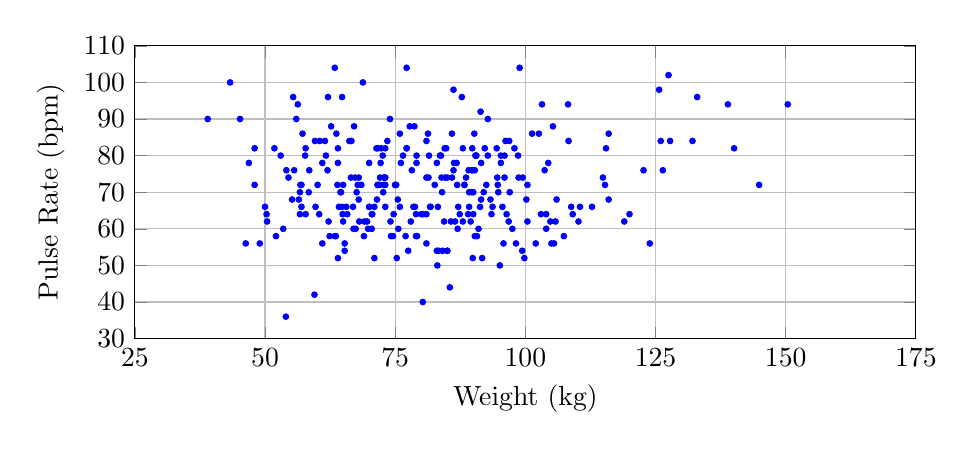
\begin{tikzpicture}
\pgfkeys{/pgf/number format/.cd,
fixed,
precision=999,
set thousands separator={},
1000 sep in fractionals=false,
}
\begin{axis}[
width=11.5cm,
height=5.3cm,
xlabel={Weight (kg)},
ylabel={Pulse Rate (bpm)},
ymajorgrids=true,
xmajorgrids=true,
%enlarge x limits=false,
%enlarge y limits=false,
xticklabel style={/pgf/number format/.cd,fixed,precision=0},
xticklabel=\pgfmathprintnumber{\tick},
xtick={25,50,...,175},
ytick={30,40,...,110},
ymin=30,
ymax=110,
xmin=25,
xmax=175,
scatter/use mapped color={
 %draw=mapped color,
 fill=blue,
},
]
\addplot[scatter, only marks, blue, scatter src=y, mark size=1pt]
coordinates
{
(	98.6	,	80.0	)
(	96.9	,	84	)
(	108.2	,	94.0	)
(	73.1	,	74.0	)
(	83.1	,	50	)
(	87	,	60.0	)
(	64	,	52.0	)
(	79.2	,	58.0	)
(	64.2	,	66.0	)
(	119	,	62	)
(	71	,	52.0	)
(	98.2	,	56.0	)
(	122.7	,	76.0	)
(	75.3	,	52.0	)
(	51.8	,	82	)
(	76.1	,	78.0	)
(	89.5	,	62.0	)
(	75.9	,	86.0	)
(	67.1	,	88.0	)
(	86.9	,	72.0	)
(	91	,	60.0	)
(	96.4	,	64	)
(	81	,	56.0	)
(	86.3	,	78	)
(	54	,	36.0	)
(	72.3	,	82.0	)
(	78.5	,	66.0	)
(	71	,	66	)
(	60.5	,	84	)
(	75.9	,	66	)
(	55.6	,	76	)
(	46.9	,	78.0	)
(	93.5	,	64.0	)
(	50	,	66.0	)
(	86.8	,	78.0	)
(	87.8	,	96.0	)
(	69.8	,	60.0	)
(	57.8	,	64.0	)
(	73.5	,	84.0	)
(	57.8	,	82.0	)
(	59.5	,	42.0	)
(	81.3	,	86	)
(	88.3	,	72.0	)
(	72.7	,	70	)
(	66.5	,	74	)
(	85.9	,	86.0	)
(	103	,	64.0	)
(	39.0	,	90.0	)
(	105.3	,	88	)
(	94.7	,	72.0	)
(	144.9	,	72.0	)
(	92.8	,	90	)
(	45.2	,	90.0	)
(	150.4	,	94.0	)
(	71.5	,	68.0	)
(	84.1	,	54.0	)
(	112.8	,	66.0	)
(	74.0	,	90	)
(	64.0	,	82	)
(	92.8	,	80.0	)
(	85.9	,	74.0	)
(	105.5	,	56.0	)
(	123.9	,	56.0	)
(	76.5	,	80.0	)
(	43.3	,	100.0	)
(	71.7	,	72.0	)
(	90.0	,	64.0	)
(	70.6	,	64.0	)
(	114.9	,	74.0	)
(	64.8	,	96.0	)
(	77	,	58.0	)
(	89.1	,	76.0	)
(	58.5	,	76.0	)
(	57.2	,	86.0	)
(	93.7	,	66.0	)
(	81.4	,	74	)
(	95.6	,	66.0	)
(	107.4	,	58.0	)
(	74.6	,	58.0	)
(	106.0	,	68.0	)
(	84	,	70.0	)
(	86.5	,	62.0	)
(	59.6	,	84.0	)
(	79.1	,	78.0	)
(	68	,	68.0	)
(	63.4	,	58.0	)
(	85.7	,	62	)
(	70	,	78.0	)
(	50.4	,	62	)
(	72.1	,	74.0	)
(	77.2	,	104.0	)
(	70	,	66.0	)
(	63.7	,	86	)
(	90	,	70.0	)
(	83.3	,	54.0	)
(	88.6	,	74.0	)
(	99.4	,	54.0	)
(	84.6	,	74.0	)
(	127.8	,	84.0	)
(	88.3	,	72.0	)
(	94.6	,	74.0	)
(	120	,	64.0	)
(	78.8	,	66.0	)
(	81.0	,	84.0	)
(	84.4	,	62.0	)
(	53.5	,	60.0	)
(	74.1	,	62.0	)
(	91.7	,	52	)
(	89.8	,	82.0	)
(	77.5	,	54.0	)
(	66.2	,	84.0	)
(	69.1	,	62	)
(	83.0	,	54.0	)
(	98.9	,	104.0	)
(	91.5	,	78.0	)
(	59.7	,	66.0	)
(	65.3	,	56.0	)
(	78.7	,	88	)
(	57	,	66.0	)
(	61.5	,	84.0	)
(	65.8	,	64.0	)
(	80	,	64.0	)
(	83.0	,	78.0	)
(	63.4	,	104.0	)
(	126.4	,	76.0	)
(	66.6	,	84.0	)
(	126.0	,	84.0	)
(	65	,	62	)
(	71.7	,	82.0	)
(	104	,	64.0	)
(	64.0	,	78	)
(	94.8	,	70.0	)
(	78.2	,	76	)
(	90.2	,	86.0	)
(	48	,	72.0	)
(	88	,	82.0	)
(	64.8	,	66.0	)
(	95.1	,	50.0	)
(	77.2	,	82.0	)
(	80.3	,	40.0	)
(	99.5	,	74.0	)
(	110.5	,	66	)
(	83.9	,	74.0	)
(	86.2	,	76.0	)
(	81.8	,	66.0	)
(	70	,	66.0	)
(	62.4	,	58.0	)
(	105.8	,	62.0	)
(	83.8	,	80.0	)
(	63.6	,	58.0	)
(	77.2	,	82.0	)
(	50.3	,	64.0	)
(	48.0	,	82	)
(	89.7	,	76	)
(	132.1	,	84.0	)
(	92.0	,	70.0	)
(	62.7	,	88	)
(	85.5	,	44.0	)
(	81	,	64	)
(	81.5	,	80.0	)
(	68.1	,	62	)
(	56.7	,	70.0	)
(	73.1	,	82.0	)
(	95.3	,	78.0	)
(	68	,	74	)
(	52.1	,	58.0	)
(	87.4	,	64.0	)
(	55.2	,	68	)
(	89.7	,	70.0	)
(	80.3	,	64.0	)
(	90.3	,	58.0	)
(	89.9	,	52	)
(	67.0	,	60.0	)
(	100.4	,	72.0	)
(	95.3	,	80.0	)
(	97.0	,	70	)
(	54.5	,	74.0	)
(	75	,	72.0	)
(	65.6	,	66.0	)
(	108.8	,	66.0	)
(	69	,	58	)
(	73.0	,	74.0	)
(	67.6	,	70.0	)
(	140.1	,	82.0	)
(	91.3	,	66.0	)
(	86.2	,	98.0	)
(	72.8	,	74.0	)
(	73.1	,	72.0	)
(	81.7	,	66.0	)
(	99.8	,	52.0	)
(	97.9	,	82.0	)
(	90.4	,	80	)
(	115.5	,	82.0	)
(	89.2	,	66.0	)
(	73.1	,	66.0	)
(	64.6	,	70.0	)
(	91.5	,	68.0	)
(	87.1	,	66.0	)
(	95.8	,	56.0	)
(	46.3	,	56.0	)
(	63.9	,	72.0	)
(	72.2	,	78.0	)
(	68.8	,	100.0	)
(	97.5	,	60.0	)
(	127.5	,	102.0	)
(	85.0	,	74	)
(	49	,	56.0	)
(	109.1	,	64.0	)
(	77.8	,	88.0	)
(	93.3	,	68.0	)
(	68.5	,	72.0	)
(	56.7	,	64.0	)
(	70.5	,	60.0	)
(	138.9	,	94.0	)
(	90.6	,	80.0	)
(	72.8	,	72.0	)
(	61	,	56.0	)
(	116	,	86.0	)
(	75.2	,	72.0	)
(	81	,	74.0	)
(	91.4	,	92.0	)
(	79	,	58	)
(	83.6	,	80.0	)
(	89.9	,	76.0	)
(	89	,	64.0	)
(	105	,	56.0	)
(	116.0	,	68.0	)
(	74.7	,	64.0	)
(	102	,	56	)
(	104.8	,	62.0	)
(	64.9	,	64.0	)
(	85	,	54.0	)
(	79.0	,	64.0	)
(	74.2	,	58.0	)
(	66.9	,	66.0	)
(	75	,	72.0	)
(	64.5	,	70.0	)
(	90.7	,	58.0	)
(	53	,	80	)
(	92.5	,	72.0	)
(	82.6	,	72.0	)
(	62.2	,	62.0	)
(	104	,	60.0	)
(	62.1	,	96.0	)
(	88	,	62.0	)
(	72	,	72.0	)
(	75.6	,	60.0	)
(	94.5	,	82.0	)
(	92.2	,	82.0	)
(	56.8	,	72.0	)
(	125.7	,	98	)
(	100.4	,	62.0	)
(	103.7	,	76.0	)
(	57	,	72.0	)
(	61.7	,	80.0	)
(	108.3	,	84.0	)
(	61.0	,	78.0	)
(	104.4	,	78.0	)
(	56.5	,	68	)
(	96.2	,	84	)
(	98.7	,	74.0	)
(	101.3	,	86.0	)
(	115.3	,	72.0	)
(	67.4	,	60.0	)
(	58.4	,	70.0	)
(	83.2	,	66.0	)
(	60.1	,	72.0	)
(	84.8	,	82.0	)
(	90.5	,	80.0	)
(	60.4	,	64.0	)
(	84.5	,	82.0	)
(	96	,	80.0	)
(	65.3	,	54	)
(	57.7	,	80.0	)
(	69.6	,	62.0	)
(	67.3	,	74.0	)
(	72.6	,	80.0	)
(	133	,	96.0	)
(	90.3	,	76.0	)
(	89.2	,	70.0	)
(	85	,	54.0	)
(	65	,	72	)
(	100.2	,	68.0	)
(	75.5	,	68.0	)
(	79.1	,	80.0	)
(	67.8	,	72	)
(	55.4	,	96.0	)
(	54.1	,	76.0	)
(	96.8	,	62.0	)
(	70.5	,	64.0	)
(	71.6	,	72	)
(	78	,	62	)
(	110.2	,	62	)
(	71.4	,	82.0	)
(	62.0	,	76.0	)
(	56.3	,	94.0	)
(	103.2	,	94.0	)
(	102.6	,	86.0	)
(	96	,	74	)
(	56	,	90.0	)
};
\end{axis}
\end{tikzpicture}
\end{center}\pause
The points do not show any obvious pattern, and this lack of a pattern suggests that there is no relationship between weights and pulse rates.
\end{example}
\end{frame}
\end{document}